\section{Preliminaries and Background}
\label{sec:prelim}

% Basics definitions and theory for this topic can be found in~\ref{sec:appendix:defs}.

We first give basic definitions and concepts in combinatorial rigidity, leading to a definition of a DR-plan, its properties, and how they relate. The section ends with a discussion of previous work on DR-plans.

\subsection{Geometric Constraint Systems and Combinatorial Rigidity}
\label{sec:prelim:defs}
\label{sec:appendix:defs}


In this paper, a \dfn{geometric constraint system} is a multivariate polynomial (usually bilinear or quadratic) system $G(x,\delta)=0$, representing constraints with parameters $\delta$ between geometric primitives in $\mathbb{R}^2$ represented collectively as $x\in \mathbb{R}^n$.
%
When the type of constraint (system) is fixed, the system is simply represented as $(G,\delta)$, where $G$ is the underlying constraint (hyper)graph $G = (V,E)$ with the vertices $V$ representing the geometric primitives in $\mathbb{R}^2$ and (hyper)edges $E$ representing the constraints, each with an associated parameter $\delta$.
%
For example, a \dfn{bar-joint system or linkage} $(G,\delta)$, is a graph $G=(V,E)$ with fixed length bars as edges,
% \footnote{Geometric constraint systems can also have inequalities in addition to equations, where the parameters in $\delta$ are small intervals of values rather than exact values.}
i.e.\ $\delta: E \rightarrow \mathbb{R}$; this represents the distance constraint system $\| x_u -x_v \|_2 = \delta_{u,v}$ for  $(u,v) \in E$, where $x_u \in \mathbb{R}^2$ represents the coordinates of $u\in V$.



In all types of geometric constraint systems we consider in this paper, a Cartesian \dfn{realization} or \dfn{solution} $G(p)$ of $(G,\delta)$ is an assignment of coordinates or Euclidean transformations (poses), $p: V \rightarrow \mathbb{R}^2$ or $\mathbb{R}^3$, to the vertices of $G$ satisfying the constraints with parameters $\delta$, modulo orientation preserving isometries (Euclidean rigid body motions).

Although the realization space itself depends on the constraint parameters $\delta$, many relevant \dfn{generic} properties of the constraint system $G(x,\delta)$ are defined to be properties of the constraint (hyper)graph $G$ and do not depend on $\delta$ (or they hold for all but a measure zero set of $\delta$ values). Many of these are properties of the Jacobian $\Delta_x G(x,\delta)$, often called the appropriate \dfn{rigidity matrix of $G$} (a matrix of indeterminates). For example, the \dfn{bar-joint rigidity matrix of the graph $G = (V,E)$} is a matrix of indeterminates representing the Jacobian of the distance map $\| x_u -x_v \|_2$  for $(u,v) \in E$. The matrix has $2$ columns per vertex in $V$ and one row per edge in $E$, where the row corresponding to edge $(u,v)$ contains the 2 coordinate indeterminates for $x_u -x_v$ (resp. $x_v-x_u$) in the 2 columns for $u$ (resp.\ $v$), i.e.\ 4 non-zero entries per row.


% XXXXXXXXX
% something has to be said along with asimow roth
% (infinitesimal rigidity implies rigidity) When the rigidity matrix has
% appropriate rank, the realizations or solutions of the corresponding
% constraint system are generically isolated and zero-dimensional if the
% constraint system has equalities and exact values for the parameters
% $\delta$. If the constraint system has inequalities, i.e, if the
% $\delta$ lie in an interval, this claim is approximate: the solutions
% are isolated small, full-dimensional  connected components.

One important property of a generic constraint system or (hyper)graph\footnote{We refer to these as properties of the constraint system or as properties of the underlying (hyper)graph interchangeably}
%that depends on the appropriate rigidity matrix of indeterminates
is \dfn{rigidity},
% (\note footnote now...),
i.e.\ the realizations or solutions of the corresponding constraint system being generically isolated and zero-dimensional.
%(if the constraint system has equalities and exact values for the parameters $\delta$).
The result by Asimow and Roth \cite{asimow1978rigidity}  shows a constraint (hyper)graph is rigid if and only if  it is generically \dfn{infinitesimally rigid}, i.e.\ the number of independent rows of its appropriate rigidity matrix is at least the number of columns less the number of rigid body motions, which is 3 for 2D bar-joint systems.
%This condition is called generic {\em infinitesimal rigidity}.

% \sidenote{If the constraint system has inequalities, i.e, if the $\delta$ lie in an interval, the definition of rigidity is approximate: the solutions are isolated small, full-dimensional  connected components.}
% generic rigidity, i.e.\ there exist at most finitely many solutions to the system at generic points,  %to the algebraic system

Geometric constraint systems can also have inequalities in addition to equations, where the parameters in $\delta$ are small intervals rather than exact values. In this case, the definition of rigidity is approximate; the solutions are isolated, small, full-dimensional connected components.

Other generic constraint system or (hyper)graph properties are mentioned here.
% (\note we refer to these as properties of the constraint
% system or as properties of the underlying (hyper)graph
% interchangeably).
A constraint (hyper)graph $G$ is \dfn{independent} if its appropriate rigidity matrix of indeterminates has independent rows (i.e.\ the determinant of some square submatrix is not identically zero).
%It is {\em rigid} if the number of independent rows of the rigidity matrix is
%at least the number of columns less the number of rigid body motions,
%which is 3 for distance constraint systems.
It is \dfn{isostatic} (\dfn{minimally rigid}, \dfn{wellconstrained}) if it is both rigid and independent.
%if the number of generically independent rows or the rank of the appropriate rigidity matrix is maximal.
%For example, the maximal rank of a bar-joint rigidity matrix is $2|V| - 3$,
%where $3$ is the number of rotational and translational degrees-of-freedom of a rigid body in $\mathbb{R}^2$.
%The graph $G$ is {\em rigid} if there exists some spanning subgraph $S\subseteq G$ such that $S$ is wellconstrained.
It is \dfn{flexible} if it is not rigid, \dfn{underconstrained} if it is independent and not rigid, or \dfn{overconstrained} if it is not independent.

Defining the combinatorial independence of a subset of edges $E'\subseteq E$ to be the independence of corresponding rows in the rigidity matrix of indeterminates, we obtain the \dfn{rigidity matroid} of a constraint (hyper)graph $G = (V,E)$.
%The 2-dimensional {\em rigidity matroid} of a constraint (hyper)graph $G = (V,E)$ is a linear matroid  on $E$,
%where a subset of edges $E' \subseteq E$ is {\em independent} in the matroid,
%if the set of corresponding rows in the appropriate rigidity matrix of indeterminates are linearly independent.
There are various results on combinatorial characterization of independence, rigidity, and rigidity matroids for different types of (hyper)graphs. For bar-joint rigidity matroids, the famous Laman's theorem \cite{laman1970graphs} states that the underlying graph is isostatic if and only if $|E| = 2|V|-3$ and $|E'| \le 2|V'|-3$ for every induced subgraph with at least 2 vertices. The result by Lovasz and Yemini \cite{lovasz1982generic} shows that all 6-vertex-connected graphs are rigid in the plane. For bar-body rigidity matroids, Tay \cite{tay1976rigidity} proved that the underlying multigraph is isostatic if and only if it can be decomposed as $3$ edge disjoint spanning trees. White and Whiteley \cite{white1987algebraic} gave the same characterization using a different technique to study the algebraic-geometric conditions of genericity, called pure condition. Lee, Streinu and Theran \cite{lee2007graded} defined the \dfn{$(k,l)$-sparsity matroid}, where a hypergraph $G$ is called \dfn{$(k,l)$-sparse} if $|E'| \le k|V'| - l$ for any induced subgraph $(V',E')$ with at least 2 vertices, and \dfn{$(k,l)$-tight} if it is $(k,l)$-sparse and $|E| = k|V| - l$. In general, given a $d$-uniform hypergraph, a $(k,l)$-sparsity condition is matroidal as long as $l \le dk-1$.

In this paper, a \dfn{qusecs} is any independent geometric constraint system of one of 3 types: bar-joint (defined formally in \ref{sec:prelim:defs}), \dfn{body-hyperpin} (defined formally in Section \ref{sec:bodypin}), and \dfn{pinned line-incidence} (defined formally in Section \ref{sec:pinnedline}).



% In this paper, a \dfn{qusecs} is any \dfn{independent} geometric constraint system of one of the 3 types mentioned above.

% % \medskip\noindent
% % \note In the remainder of this section and sections~\ref{sec:DRP} and \ref{sec:recomb} we only consider bar-joint qusecs and graphs. Relevant formal analogies for the other 2 types of qusecs and (hyper)graphs are given in the subsequent 2 sections on Applications.

% \sidenote{In the remainder of this section and Sections~\ref{sec:DRP} and \ref{sec:recomb} we only consider bar-joint qusecs and graphs. Relevant formal analogies for the other 2 types of qusecs and (hyper)graphs are given in the subsequent 2 sections on Applications (\ref{sec:bodypin} and \ref{sec:pinnedline}).}



%XXXNow comes the definition of stress vector and flex vector.
%NOTE: something has to be said about what flexes and stresses mean


%TODO
%Given a bar-joint graph, a vector (of indeterminates) in the right null space of its rigidity matrix is called a \dfn{flex vector}. It has 2 entries per vertex and represents the internal motions of the system (i.e.\ modulo rigid body motions). For rigid graphs, all flex vectors are identically zero.
%
%A vector (of indeterminates) in the left null space of the rigidity matrix is called a \dfn{stress vector}. It has one entry per edge and represents a \dfn{self stress} of the system. For independent graphs, all stress vectors are identically zero.
%
%An \dfn{external stress} $t$ is a $1\times 2|V|$ vector  (of indeterminates) which specifies a 2D vector acting at each vertex such that the stress balance equation $sR = t$ holds, where $s$ is a vector of internal stresses, one for each bar, and $R$ is the rigidity matrix.




%\subsection{Qusecs}


% \medskip\noindent
% \note In the remainder of this section and sections~\ref{sec:DRP} and \ref{sec:recomb} we only consider bar-joint qusecs and graphs. Relevant formal analogies for the other 2 types of qusecs and (hyper)graphs are given in the subsequent 2 sections on Applications.

We note that  the remainder of this section and Sections~\ref{sec:DRP} and \ref{sec:recomb} we only consider bar-joint qusecs and graphs. Relevant formal analogies for the other 2 types of qusecs and (hyper)graphs are given along with their materials applications in Sections \ref{sec:bodypin} and \ref{sec:pinnedline}.






\subsection{Decomposition-Recombination (DR-) Plans}
%
%$G=(V,E,w_V,w_E)$ is a set of vertices, $V$, and a set of edges, $E$, defined as a tuple of vertices from $V$ (undirected). Additionally, there are two weight functions, $w_V: V \to \mathbb{R}^+$ and $w_E: E \to \mathbb{R}^+$. The \textbf{density} of graph $G$ is $d(G) = \sum_{e\in E}{w_E(e)} - \sum_{v\in V}{w_V(v)}$.
%
%Given a constant $k$, a graph $G$ is:
%\begin{itemize}
%    \item \textbf{independent} (or \textbf{sparse}) if, for all non-trivial subgraphs $S\subseteq G$, $d(S) \leq k$.
%
%    \item \textbf{overconstrained} if it is not independent.
%
%    \item \textbf{wellconstrained} (or \textbf{tight}) if $G$ is independent and $d(G)=k$.
%
%    \item \textbf{rigid} if there exists some spanning subgraph $S\subseteq G$ such that $S$ is wellconstrained.
%
%    \item \textbf{underconstrained} if $G$ is independent and not rigid.
%
%    % \item \textbf{trivial} if (1) it is overconstrained graph and (2) all of its subgraphs are also trivial. Trivial graphs are input.
%\end{itemize}
%
% \begin{definition}
%     A graph is \textbf{overconstrained} if, given constant $k$, there exists some
%     % induced
%     subgraph $S\subseteq G$ such that $d(S) > k$.
% \end{definition}
%
% \begin{definition}
%     A graph is \textbf{wellconstrained} if, given constant $k$, $d(G) = k$ and for all
%     % induced
%     subgraphs $S\subseteq G$, (1) $d(S)\leq k$, or (2) given a set of trivial graphs $T$, $S$ is isomorphic to one of the graphs in $T$ (i.e.\ $S$ is trivial).
% \end{definition}
%
%
%
% \begin{definition}
%     A \textbf{trivial} graph is ill-defined in the general case. The only strict requirements are: (1) it must be an overconstrained graph and (2) all of its subgraphs are also trivial.
%     \todo{Maybe leave the following out until it's needed later?}
%     In the familiar geometric cases of $d$-dimensional space, all vertex weights are $d$, all edge weights are $1$, and constant $k= -{{d+1}\choose{2}}$. Trivial graphs for 2D would be a single vertex. Trivial graphs in 3D would be a vertex and an edge (2 vertices with an edge between). Etc. These trivial graphs capture the notion of the rotational symmetry that exists in geometric spaces.
% \end{definition}
%


% \ClearMyMinHeight
% \SetMyMinHeight{.4}{../../img/epsfromtikz/demo_graph}
% \SetMyMinHeight{.3}{../../img/epsfromtikz/demo_graph_comdrp}
% \SetMyMinHeight{.3}{../../img/epsfromtikz/demo_graph_candrp}

% \begin{figure*}\centering%
%   %
%   \begin{subfigure}{0.4\linewidth}\centering
%     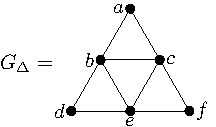
\includegraphics[height=\myMinHeight]{../../img/epsfromtikz/demo_graph}
%     \caption{}\label{fig:demo_graph:graph}
%   \end{subfigure}%
%   %
%   \hfill
%   \begin{subfigure}{0.3\linewidth}\centering
%     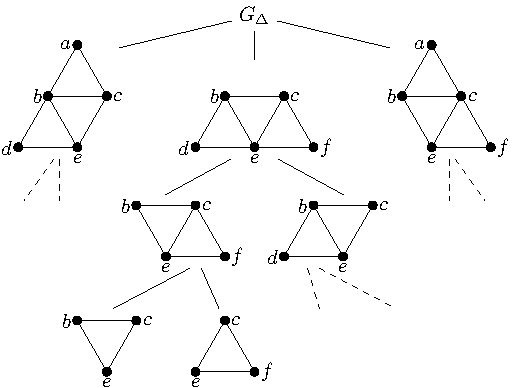
\includegraphics[height=\myMinHeight]{../../img/epsfromtikz/demo_graph_comdrp}
%     \caption{}\label{fig:demo_graph:comdrp}
%   \end{subfigure}%
%   %
%   \hfill
%   \begin{subfigure}{0.3\linewidth}\centering
%     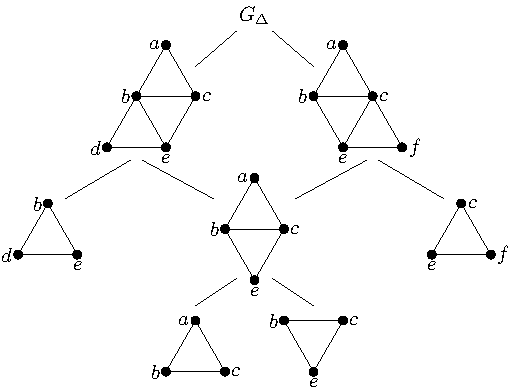
\includegraphics[height=\myMinHeight]{../../img/epsfromtikz/demo_graph_candrp}
%     \caption{}\label{fig:demo_graph:candrp}
%   \end{subfigure}%
%   %
%   \caption{(\ref{fig:demo_graph:graph}) A simple graph, $G_{\Delta}$, used to illustrate concepts throughout this and the next section. (\ref{fig:demo_graph:comdrp}) The complete DR-plan of $G_{\Delta}$, i.e.\ $ComDRP(G_{\Delta})$. Dashed lines indicate that the children repeat the same pattern as the others shown on this level. The children of triangles (3 edges) are omitted. (\ref{fig:demo_graph:candrp}) The canonical DR-plan of $G_{\Delta}$, which is optimal (see Section~\ref{sec:DRP}), i.e.\ $OptDRP(G_{\Delta})$. The children of triangles are omitted.}
%   \label{fig:demo_graph}
% \end{figure*}%



% \begin{figure*}\centering%
%   %
%   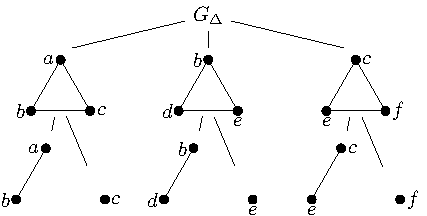
\includegraphics[width=0.4\linewidth]{../../img/epsfromtikz/demo_graph_clustmindrp}
%   \caption{A DR-plan of $G_{\Delta}$ from Figure~\ref{fig:demo_graph:graph}, which gives cluster minimality. Using the ideas from the paper~\cite{lomonosov2004graph}, the children of a triangle are the primitives of a point and an edge. Thus, the fan-in of this graph is 3, whereas the optimal DR-plans shown in Figure~\ref{fig:demo_graph:candrp} and \ref{fig:demo_graph:candrpseq} have fan-in of 2. With this counterexample, it is clear that cluster minimality is not sufficient for optimality.}
%   \label{fig:demo_graph:clustmindrp}
% \end{figure*}%



\ClearMyMinHeight
\SetMyMinHeight{.4}{../../img/svg/3xc2c3_new}
\SetMyMinHeight{.3}{../../img/svg/3xc2c3_new_comdrp}
\SetMyMinHeight{.3}{../../img/svg/3xc2c3_new_candrp}

\begin{figure*}\centering%

  \begin{subfigure}{0.4\linewidth}\centering
    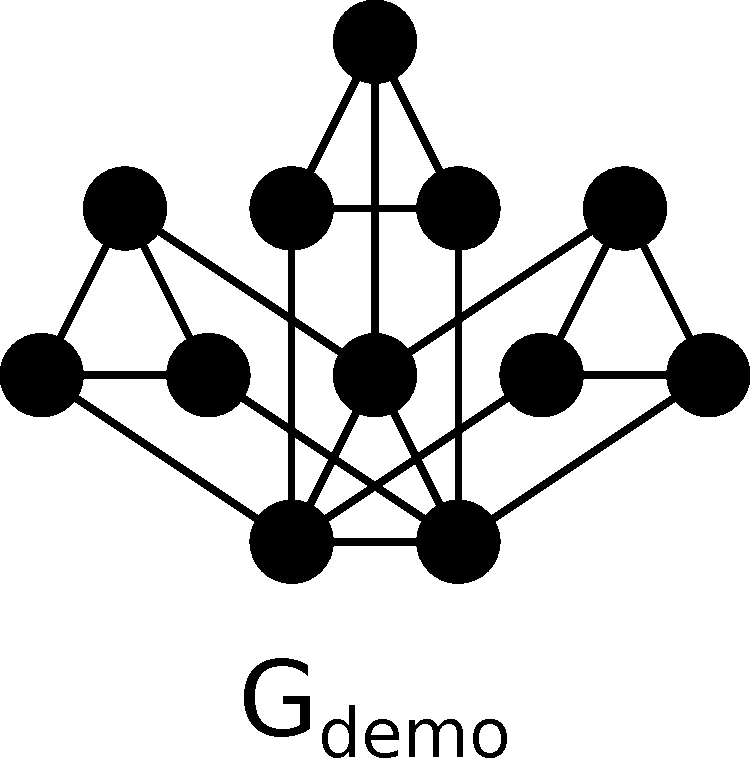
\includegraphics[height=\myMinHeight]{../../img/svg/3xc2c3_new}
    \caption{}\label{fig:demo_graph:graph}
  \end{subfigure}%
  %
  \hfill
  \begin{subfigure}{0.3\linewidth}\centering
    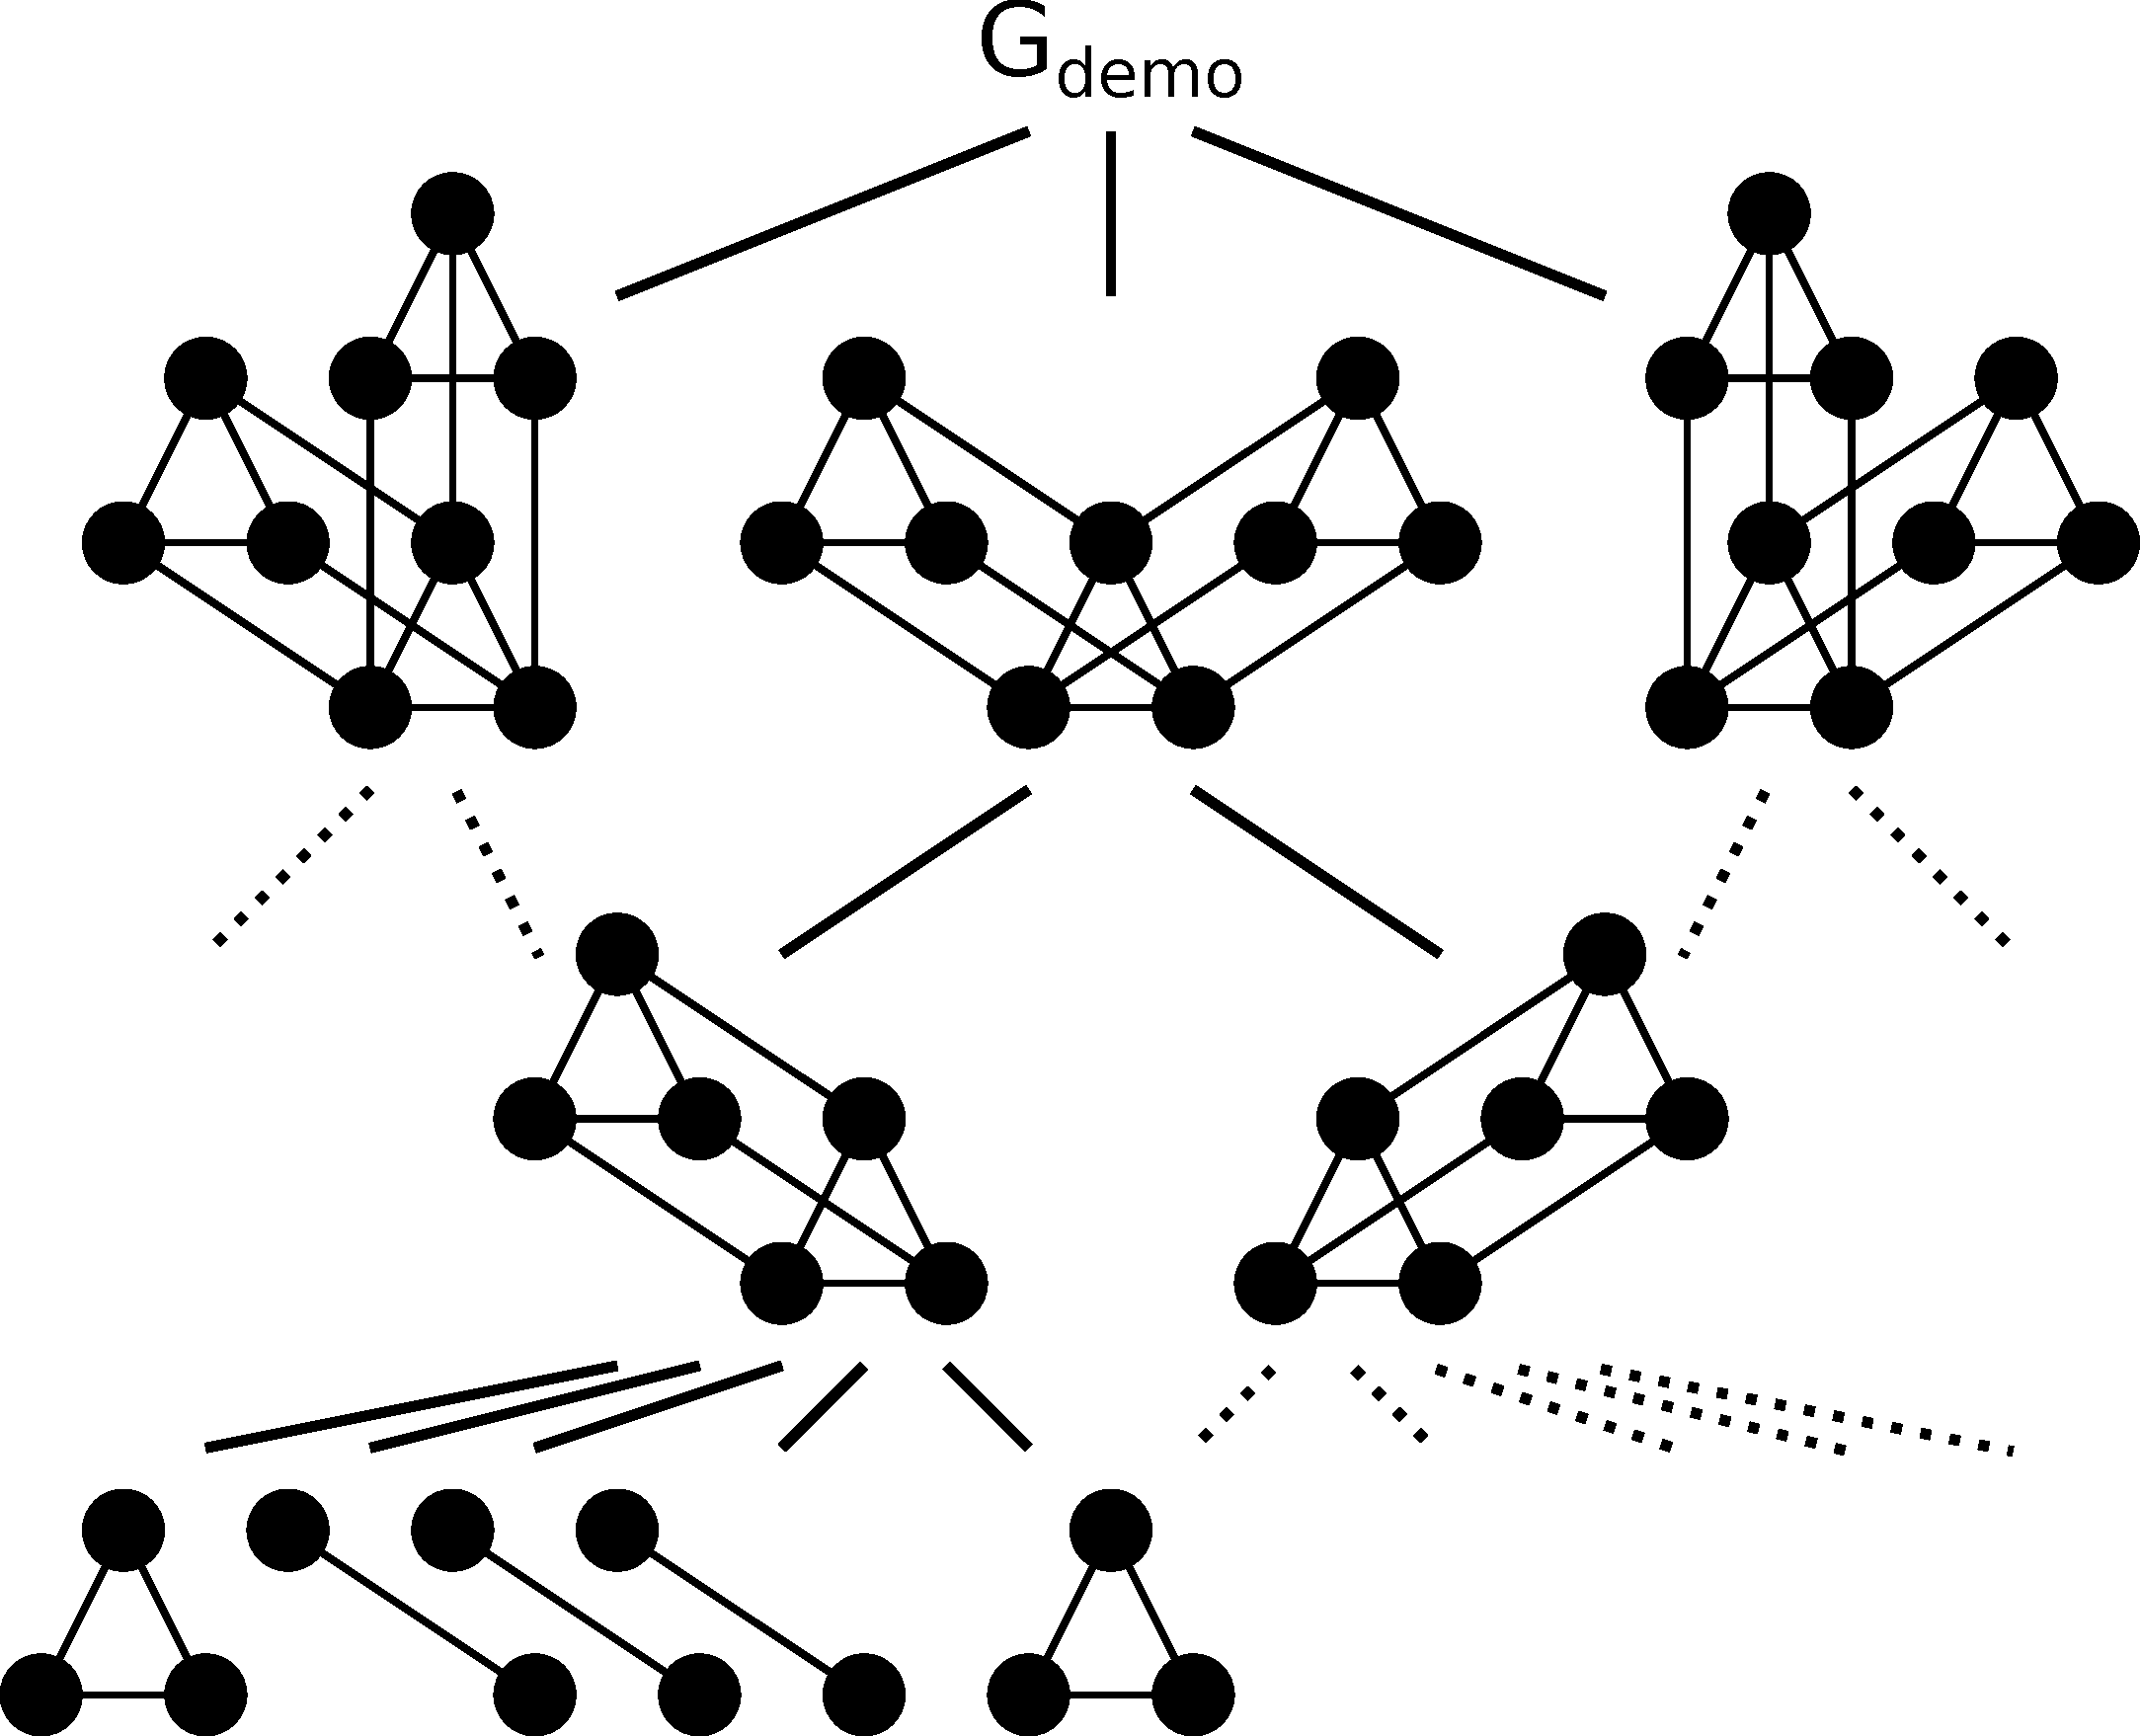
\includegraphics[height=\myMinHeight]{../../img/svg/3xc2c3_new_comdrp}
    \caption{}\label{fig:demo_graph:comdrp}
  \end{subfigure}%
  %
  \hfill
  \begin{subfigure}{0.3\linewidth}\centering
    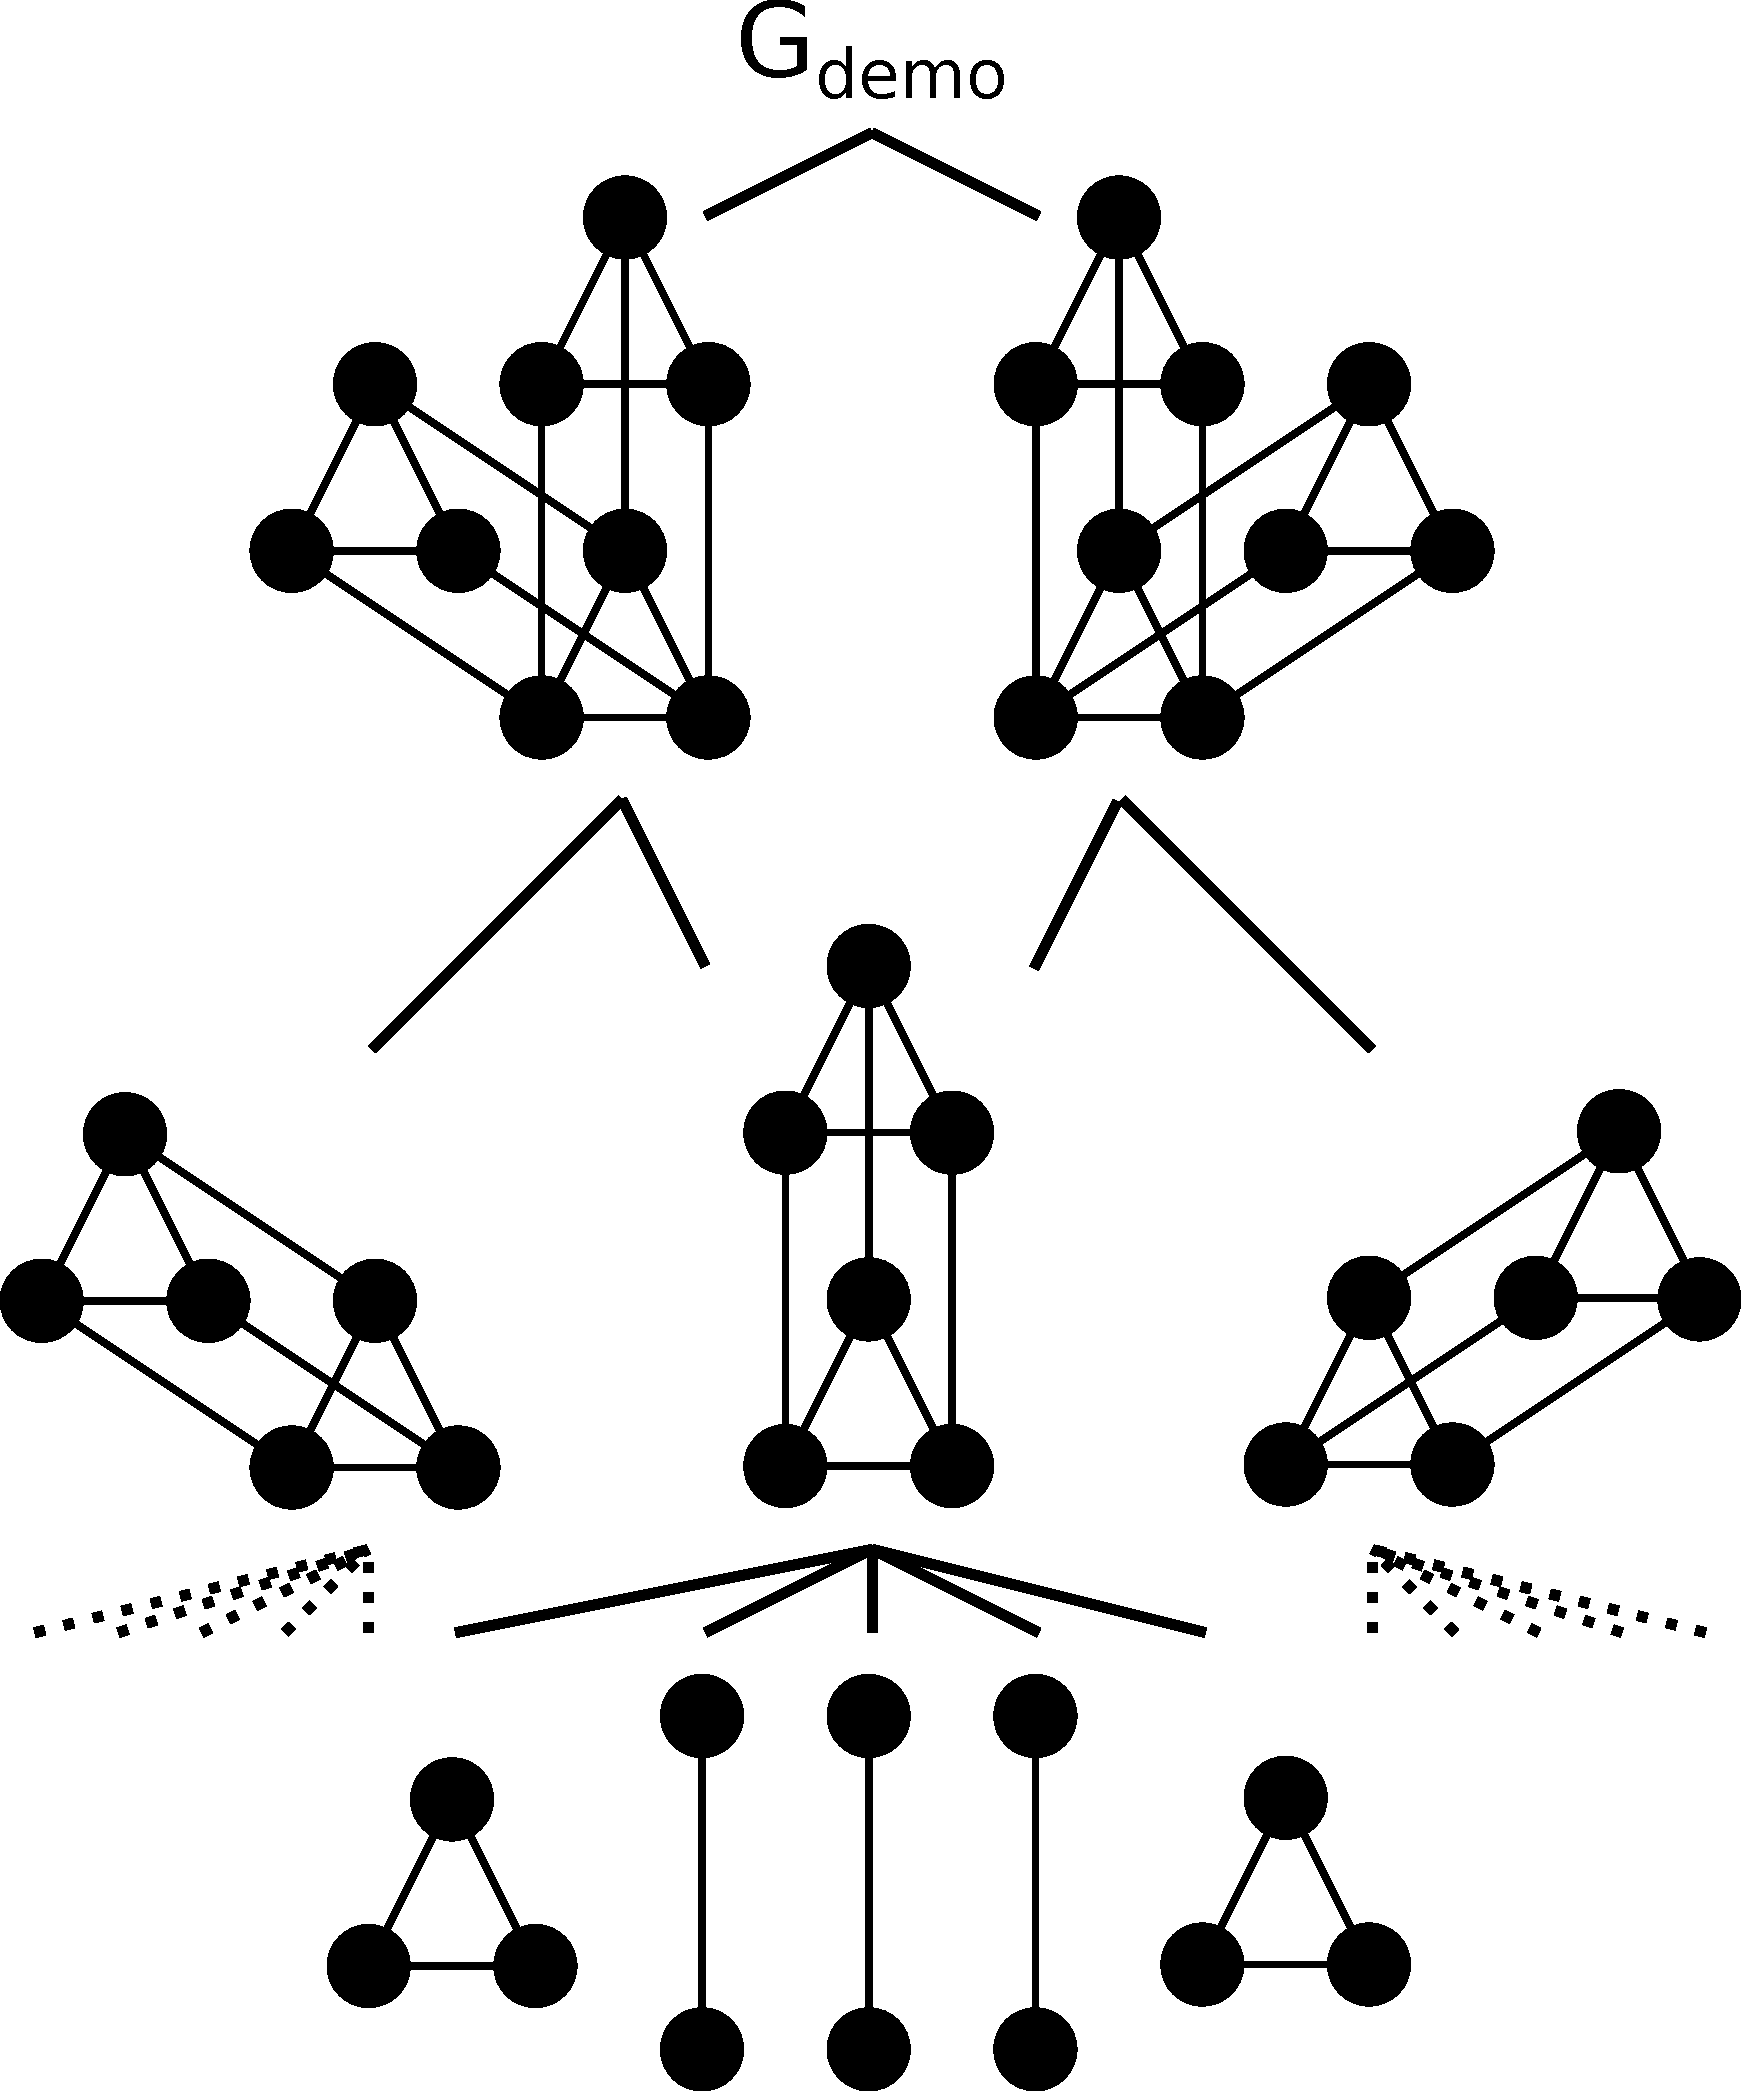
\includegraphics[height=\myMinHeight]{../../img/svg/3xc2c3_new_candrp}
    \caption{}\label{fig:demo_graph:candrp}
  \end{subfigure}%
  %
  % \begin{subfigure}[c]{0.3\linewidth}\centering
  %   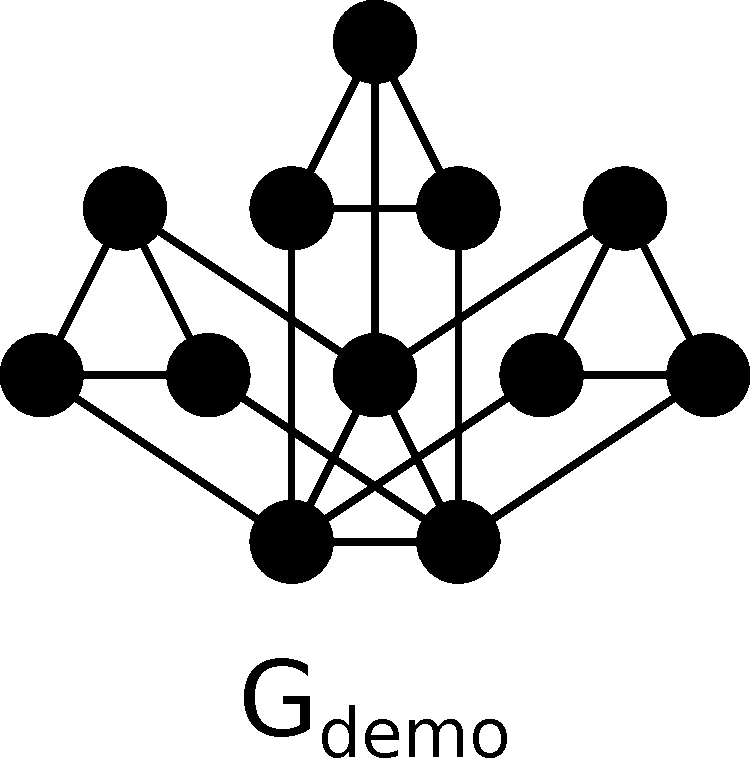
\includegraphics[width=\linewidth]{../../img/svg/3xc2c3_new}
  %   \caption{}\label{fig:demo_graph:graph}
  % \end{subfigure}%
  % %
  % \hfill
  % \begin{subfigure}[t]{0.345\linewidth}\centering
  %   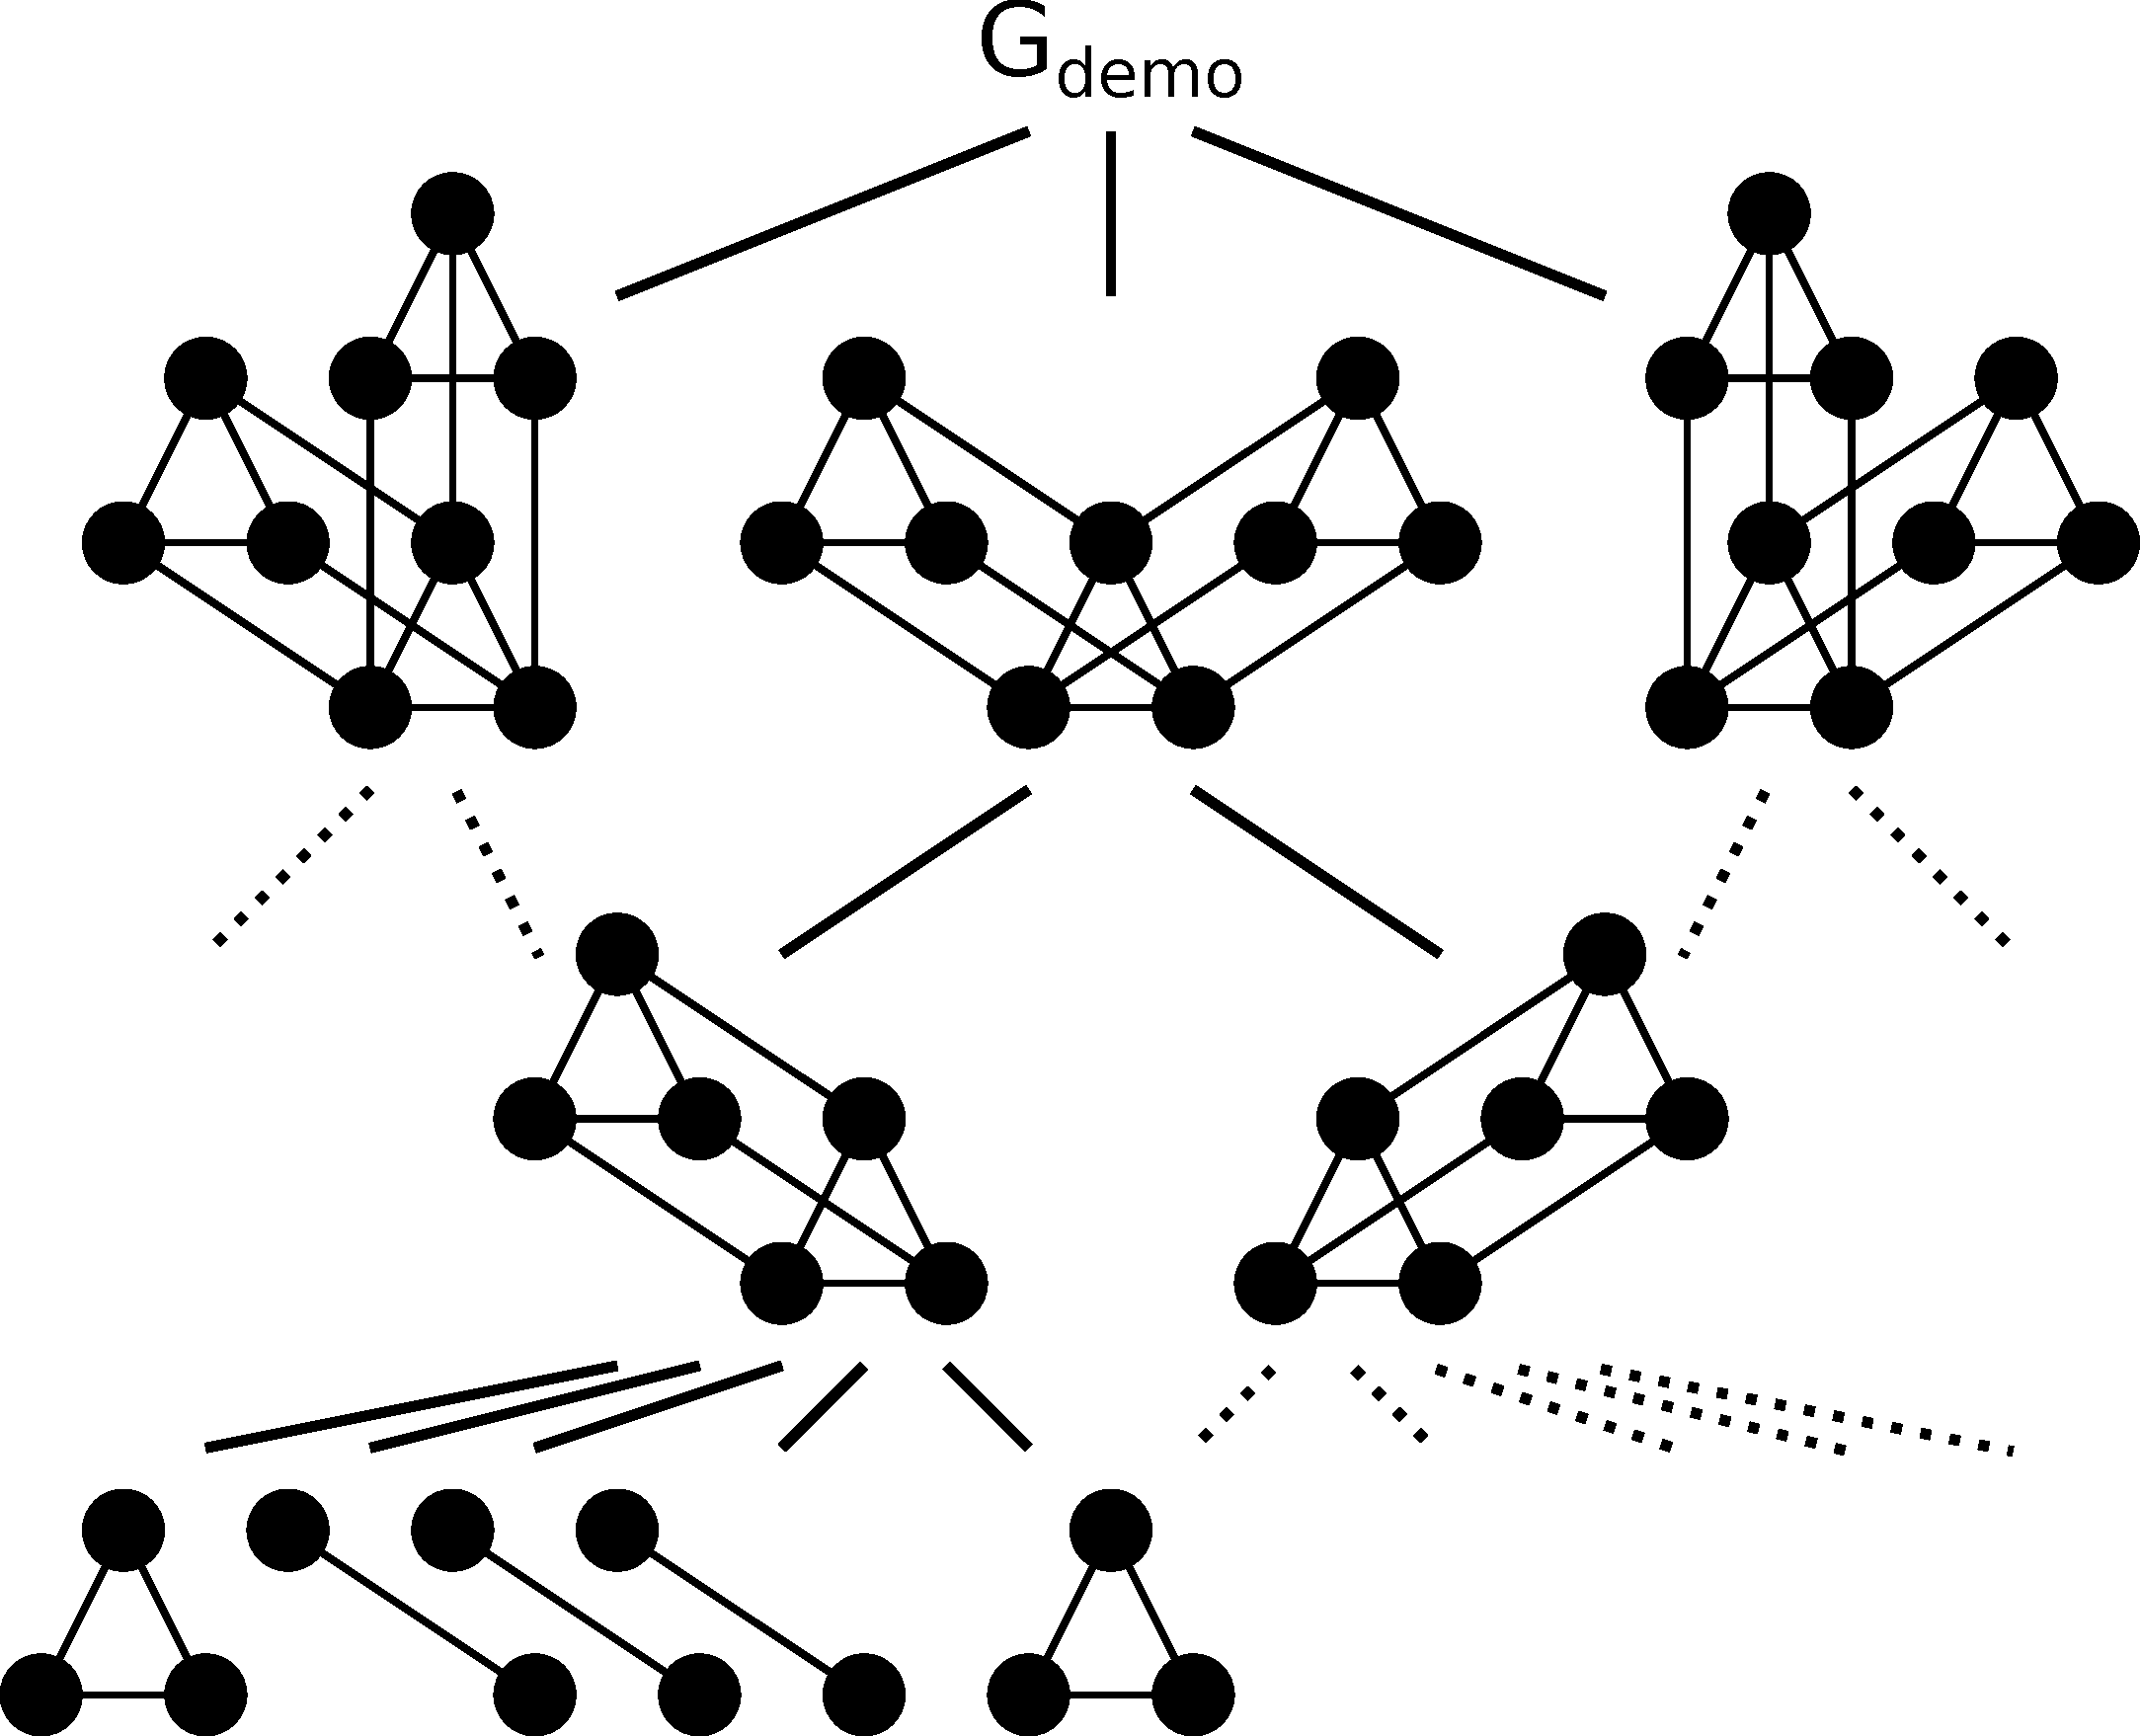
\includegraphics[width=\linewidth]{../../img/svg/3xc2c3_new_comdrp}
  %   \caption{}\label{fig:demo_graph:comdrp}
  % \end{subfigure}%
  % %
  % \hfill
  % \begin{subfigure}[t]{0.345\linewidth}\centering
  %   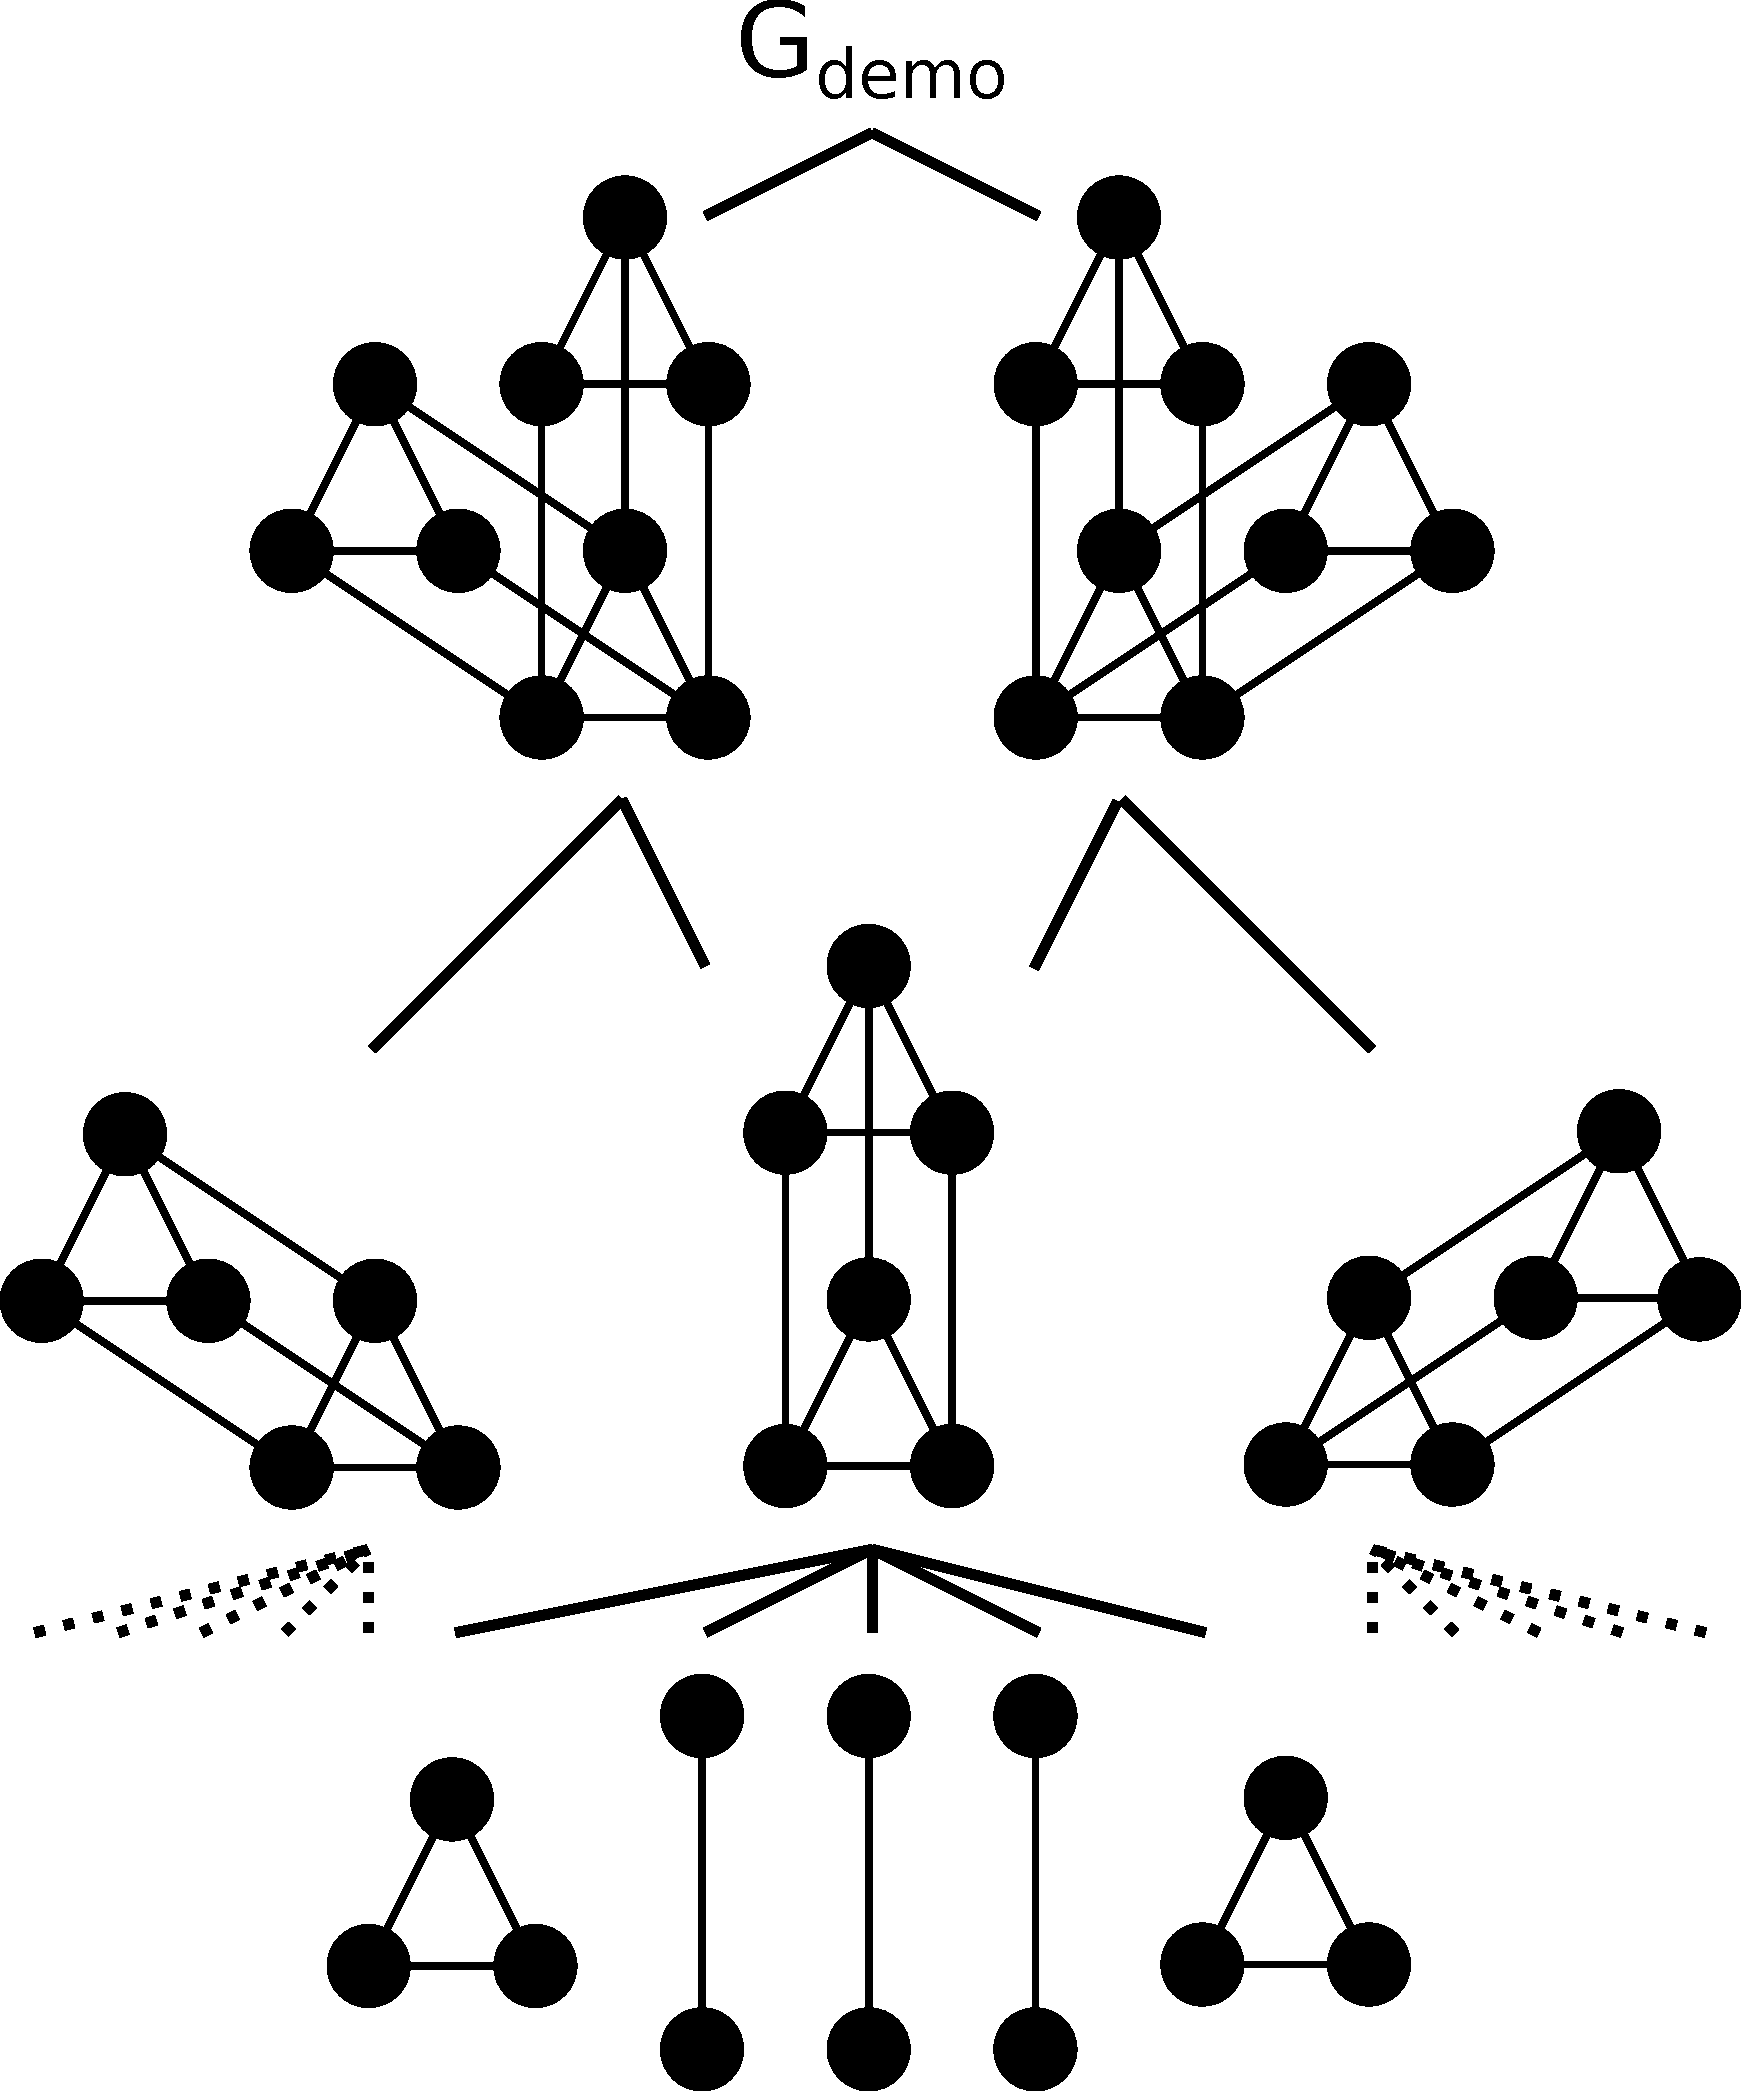
\includegraphics[width=\linewidth]{../../img/svg/3xc2c3_new_candrp}
  %   \caption{}\label{fig:demo_graph:candrp}
  % \end{subfigure}%
  %
  \caption{
  (\ref{fig:demo_graph:graph}) A graph, $G_{demo}$, used to illustrate concepts throughout this and the next section.
  %
  (\ref{fig:demo_graph:comdrp}) The complete DR-plan of $G_{demo}$.
  % i.e.\ $ComDRP(G_{demo})$.
  Dashed lines indicate that the children repeat the same pattern as the others shown on this level. The children of triangles (3 edges) are omitted.
  %
  (\ref{fig:demo_graph:candrp}) The canonical DR-plan of $G_{demo}$, which is optimal (see Section~\ref{sec:DRP}).
  % i.e.\ $OptDRP(G_{demo})$.
  The children of triangles are omitted.}
  \label{fig:demo_graph}
\end{figure*}%



% \ClearMyMinHeight
% \SetMyMinHeight{.4}{../../img/svg/triangle}
% \SetMyMinHeight{.3}{../../img/svg/triangle_candrp}
% \SetMyMinHeight{.3}{../../img/svg/triangle_clustmindrp}

%\begin{figure*}\centering%
%
%\begin{subfigure}{0.4\linewidth}\centering
%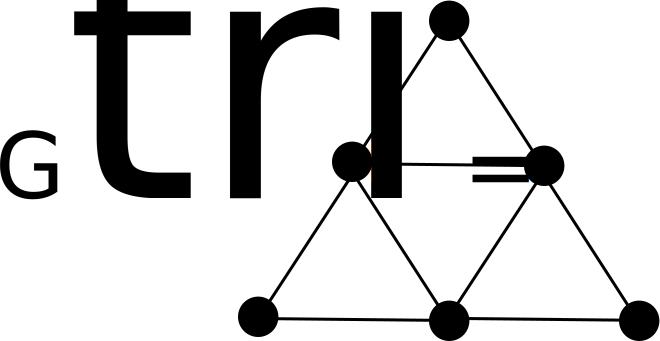
\includegraphics[height=\myMinHeight]{../../img/svg/triangle}
%    \caption{}\label{fig:demo_graph_tri:graph}
% \end{subfigure}%
%
%  \hfill
% \begin{subfigure}{0.3\linewidth}\centering
%   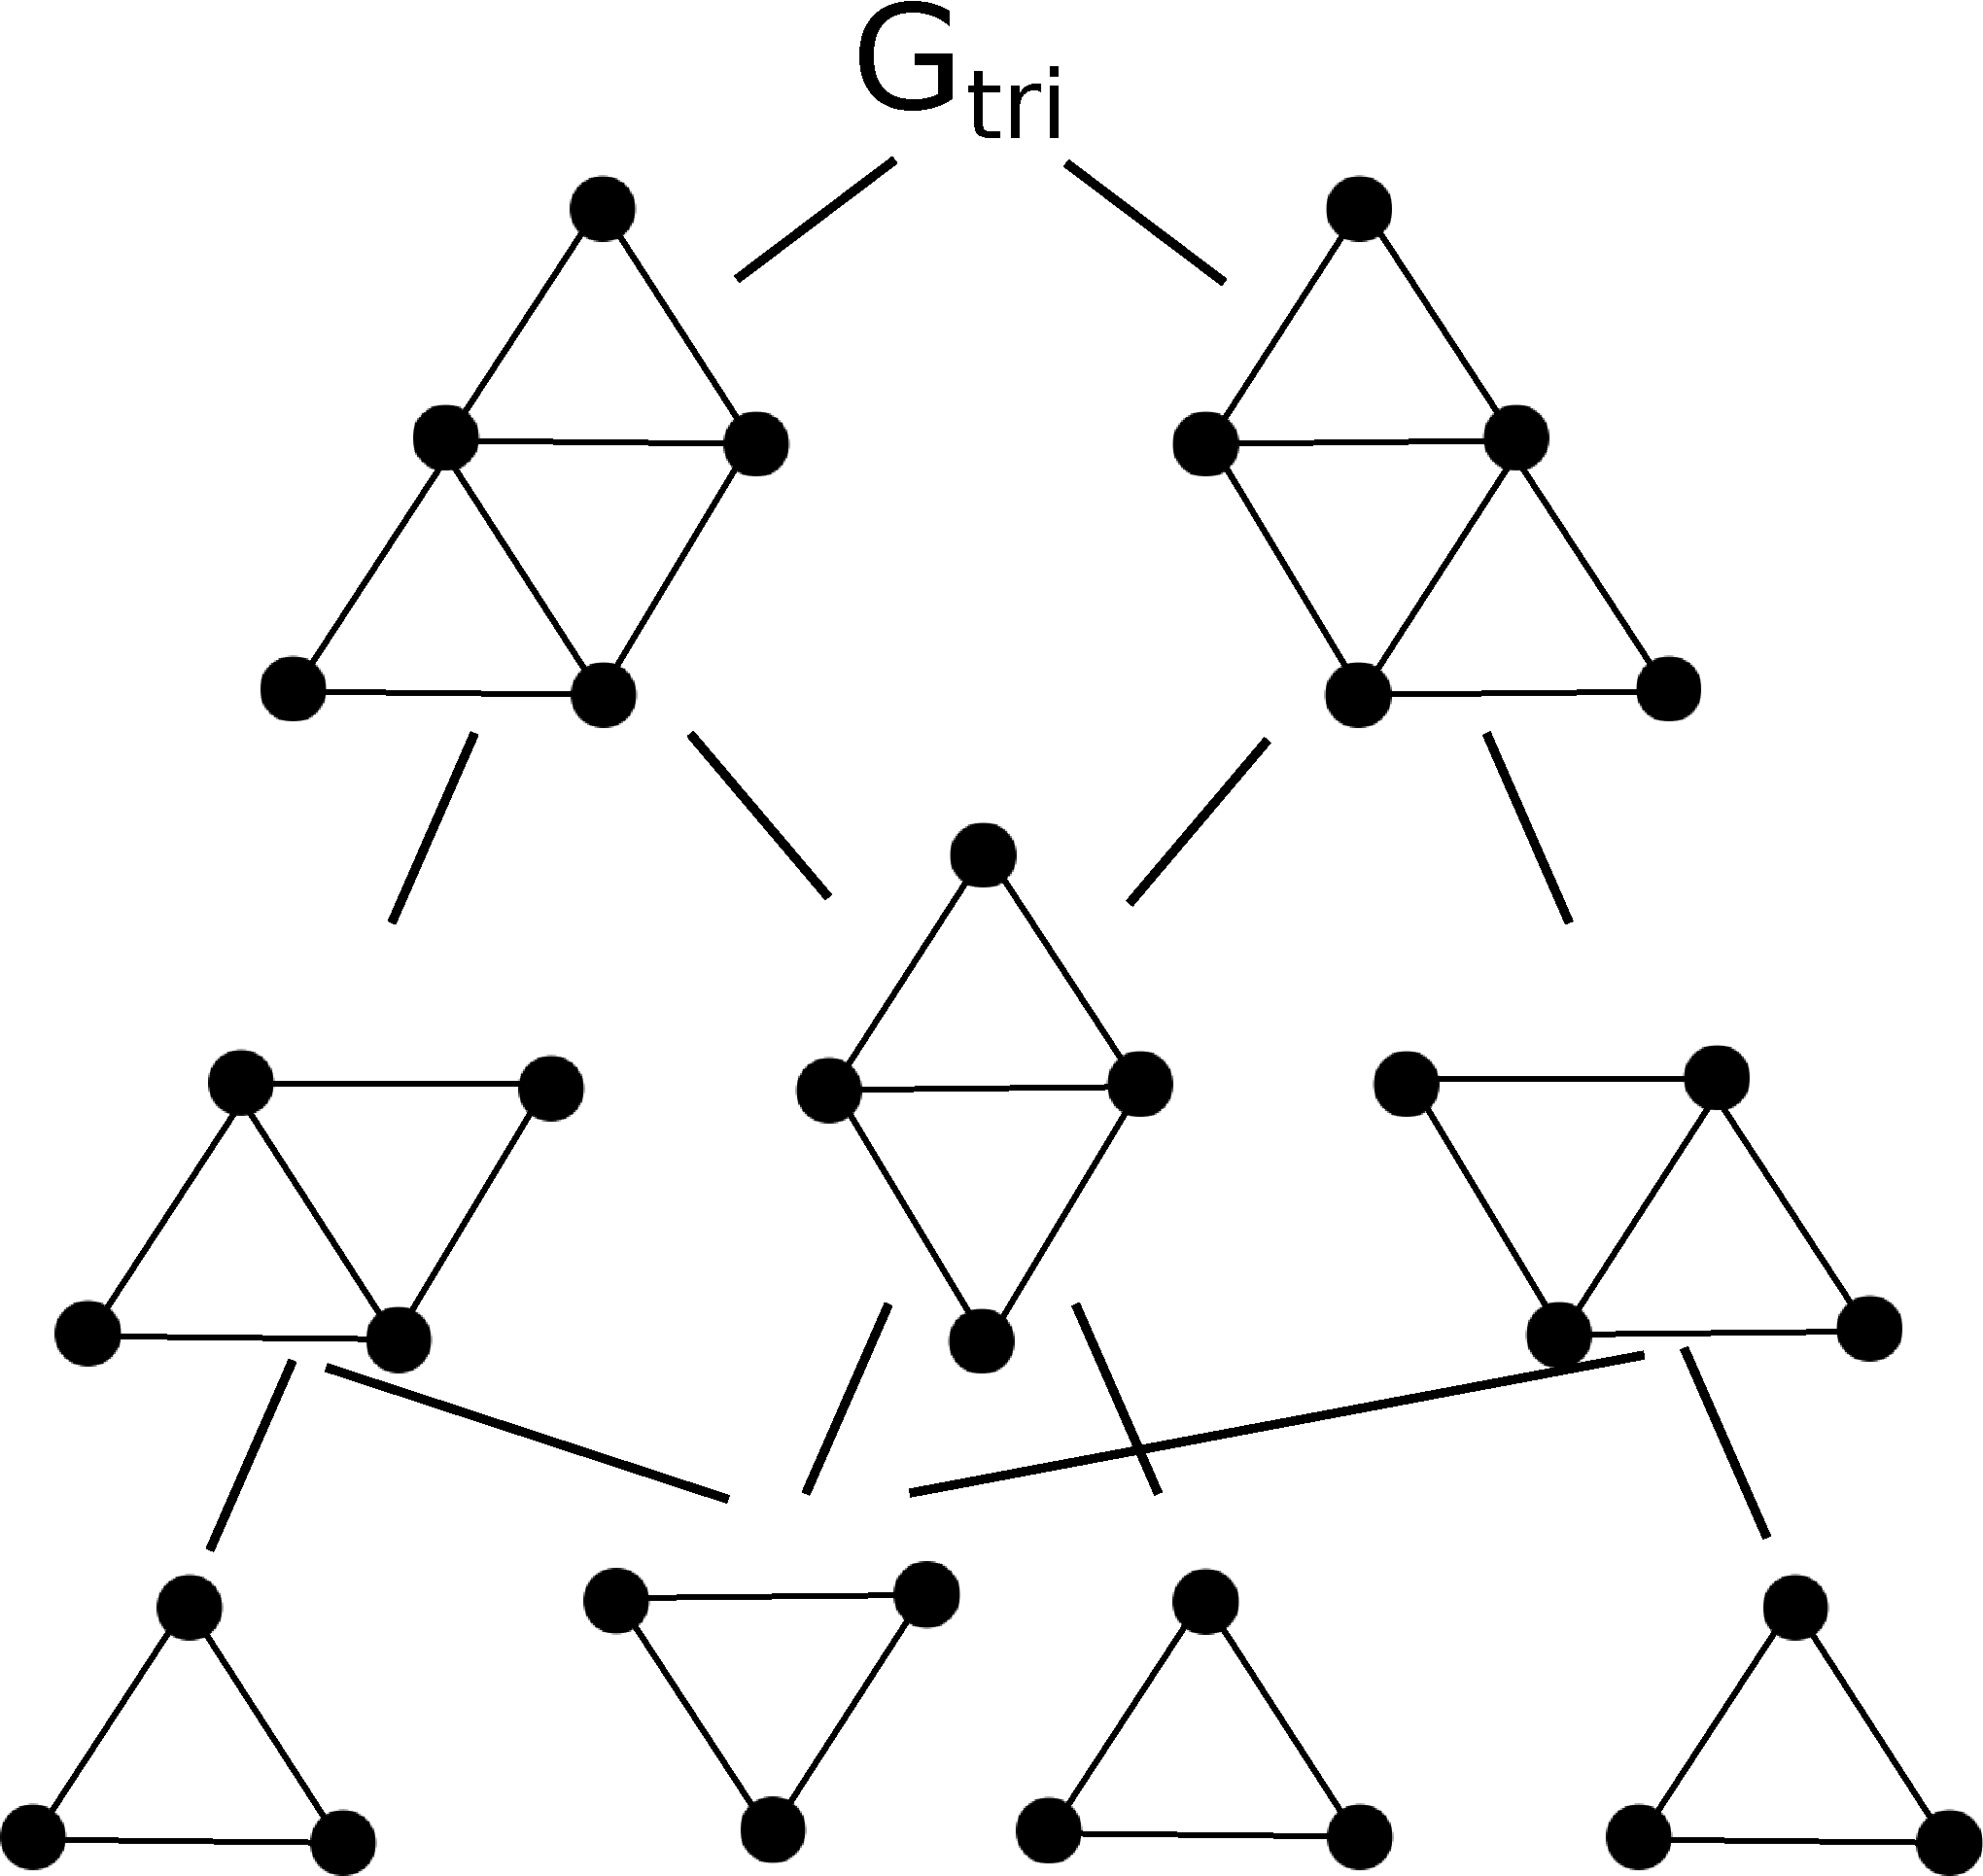
\includegraphics[height=\myMinHeight]{../../img/svg/triangle_candrp}
%    \caption{}\label{fig:demo_graph_tri:candrp}
%  \end{subfigure}%
%
%  \hfill
%  \begin{subfigure}{0.3\linewidth}\centering
%   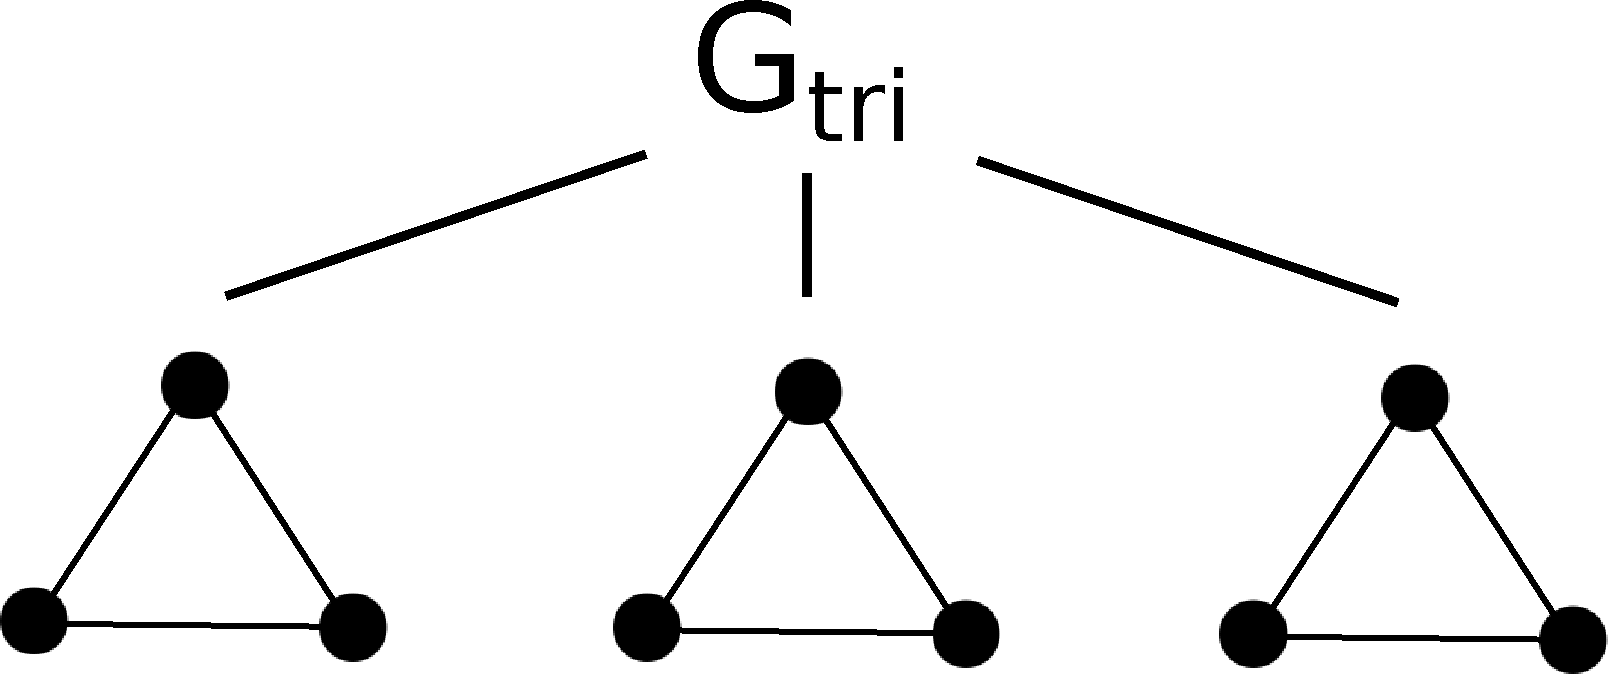
\includegraphics[height=\myMinHeight]{../../img/svg/triangle_clustmindrp}
%   \caption{}\label{fig:demo_graph_tri:clustmindrp}
%  \end{subfigure}%
%
%  \caption{(\ref{fig:demo_graph_tri:graph}) A simple graph, $G_{tri}$, of 3 triangles intersecting trivially. (\ref{fig:demo_graph_tri:candrp}) The canonical DR-plan of $G_{tri}$. (\ref{fig:demo_graph_tri:clustmindrp}) A DR-plan of graph $G_{tri}$ which gives cluster minimality  (See Section \ref{sec:prev}). Using the ideas from the paper~\cite{lomonosov2004graph}, the children of a triangle are the primitives of a point and an edge. Thus, the fan-in of this graph is 3, whereas the canonical/optimal DR-plan has fan-in of 2. With this counterexample, it is clear that cluster minimality is not sufficient for optimality.}
% \label{fig:demo_graph:clustmindrp}
%  \label{fig:demo_graph_tri}
%\end{figure*}%






% \begin{definition}\label{def:drp}
%     The \dfn{decomposition-recombination \mbox{(DR-)} plan} \cite{hoffman2001decompositionI} of graph $G$, $\drp{G}$, is defined as a forest that has the following properties:
%     \begin{enumerate}
%         \item Each node represents/contains/is a rigid subgraph of $G$.
%         % \item For a node, $C$, that is  a non-trivial graph, its $N$
%         % children, $C_1, \ldots, C_N$, are rigid vertex-maximal proper
%         % subgraphs of $C$.
%         \item The children $C_1,\ldots,C_N$ of a node $C$ satisfy $\bigcup_{i=1}^N{C_i}=C$.
%         \item A leaf node is a single edge. A \dfn{trivial} graph is empty or a single vertex. Note that a trivial graph is not isostatic.
%         \item A root node is a vertex-maximal rigid subgraph of $G$.
%     \end{enumerate}
% %
%     % It can also be described recursively as: the root is $G$, its children are the trivial subgraphs and the DR-plans of its wellconstrained vertex-maximal proper subgraphs whose union is $G$ itself.
% %
%     A DR-plan is \dfn{complete} if it satisfies an additional property: for an internal node $C$, its children are all of the rigid vertex-maximal proper subgraphs of $C$. This makes Property 2 implicit.
%   %and in fact, $C$ contains all the edges in the union of its children as well.
%   We denote a complete DR-plan of $G$ as $\comdrp{G}$.

%   A DR-plan is \dfn{optimal} if it minimizes the maximum fan-in over all nodes in the forest. The maximum  fan-in is called the \dfn{size} of the DR-plan. We denote an optimal DR-plan of $G$ as $\optdrp{G}$.
% %
% %In general, $C$ is the graph in an arbitrary node in $CompleteDRP(G)$.
% %$C_i$ is the $i^{\text{th}}$ child of $C$. It is implied that $C_i$ is
% %an isostatic vertex-maximal proper subgraph.
%     %Note that nodes will be referred to interchangeably as ``the node that
%     %represents or contains the (sub)graph $C$'' and as simply ``$C$''.
% \end{definition}



\begin{definition}
[DR-plan]
\label{def:drp}
    A \dfn{decomposition-recombination \mbox{(DR-)} plan}~\cite{hoffman2001decompositionI} of graph $G$ is defined as a forest that has the following properties:
    \begin{enumerate}
        \item Each node represents a rigid subgraph of $G$.\footnote{Nodes will be referred to interchangeably as ``the node that represents or contains the (sub)graph $C$'' and as simply ``$C$''.}
        \item A root node is a vertex-maximal rigid subgraph of $G$.
        \item A node is the subgraph of $G$ induced by the union of its children.
        \item A leaf node is a single edge.
    \end{enumerate}
\end{definition}

Note that this definition permits the same rigid subgraph to appear in multiple nodes of the DR-plan. Not permitting such duplication would, in general, require the DR-plan to be defined as a directed acyclic graph instead of a forest.

\begin{definition}
[Complete DR-plan]
    A DR-plan is \dfn{complete} if it satisfies an additional property: for an internal node $C$, its children are all of the rigid vertex-maximal proper subgraphs of $C$ (which makes Property 3 of a DR-plan implicit).
\end{definition}

\begin{definition}
[Optimal DR-plan]
    A DR-plan is \dfn{optimal} if it minimizes the maximum fan-in over all nodes in the forest.
    % The maximum fan-in is called the \dfn{size} of the DR-plan.
\end{definition}

% We denote these different kinds of DR-plans as $\drp{G}$, $\comdrp{G}$, and $\optdrp{G}$, respectively.





%
% \todo{This was labeled as both begin(remark) and end(observation), what was your intent?}
\begin{remark}
  More than one node (leaf) in a DR-plan forest may represent the same subgraph (vertex) of $G$.
  For a given graph, there could be exponentially many DR-plans -- and even optimal DR-plans -- in the size of the graph. A complete DR-plan is unique but may not be (and is usually not) optimal. DR-plans of self-similar graphs are self-similar.
\end{remark}

See Figures \ref{fig:demo_graph}, \ref{fig:c2c3ofk33s}, \ref{fig:overconstrained}, and \ref{fig:bodypindrp} for examples of DR-plans and how their properties relate to each other.


\subsection{Previous Work on DR-Plans}
\label{sec:prev}
% \todo{We now briefly survey existing techniques for studying 2D qusecs,  many of which are \dfn{bar-joint} systems (Examples 1 and 2 above, see Sections \ref{sec:prelim}, \ref{sec:DRP}, and \ref{sec:recomb}), \dfn{body-hyperpin} systems (Example 4 and 5, see Section \ref{sec:bodypin}) or \dfn{pinned-line incidence} systems (Example 3, see Section \ref{sec:pinnedline}). The limitations of these techniques directly motivate the contributions of this paper.}
We now briefly survey existing techniques for detecting rigidity and creating DR-plans of 2D constraint systems. The limitations of these techniques directly motivate the contributions of the next  section.

\subsubsection{Finding (Vertex)-Maximal, Generically Rigid Subsystems}
Fast, graph-based algorithms exist (pebble-game~\cite{Jacobs:1997:PG,hoffmann1997solvablesubsets,jermann2006decomposition,Lee:2007:PGA}), for locating all maximal, \dfn{generically rigid} subsystems \seedefs. When the input itself is rigid, these algorithms do nothing, i.e.\ compute the identity function.

However, both for self-similar or just aperiodic 2D qusecs, it is imperative to recursively decompose rigid systems into their rigid subsystems, down to the level of geometric primitives, in order to understand or design properties at all scales, such as \seedefs\ \dfn{rigidity}, \dfn{flexes}, distribution of \dfn{external stresses}, boundary conditions for \dfn{isostaticity}, as well as behavior under constraint variations.

\subsubsection{Optimal Recursive Decomposition (DR-Planning)}
Recursive decomposition of geometric constraint systems has been formalized \cite{hoffman2001decompositionI,hoffman2001decompositionII} and well-studied \cite{lomonosov2004graph,sitharam2005combinatorial,jermann2006decomposition} as the \dfn {Decomposition-Recombination (DR-) planning} problem \seedefsprelim. For the abovementioned classes of 2D qusecs, generic rigidity is a combinatorial property and hence each level of the decomposition should, in principle, be achievable by a graph-based algorithm without involving the geometric information in the constraint system. Since many such decompositions can exist for a given constraint system, criteria defining desirable or optimal DR-plans and DR-planning algorithms were given in~\cite{hoffman2001decompositionI}.
%
We conjecture (in Section~\ref{sec:open}) that one such decomposition, a version of \frontier~\cite{hoffman2001decompositionI, hoffman2001decompositionII,lomonosov2004graph,sitharam2005combinatorial}, which is a bottom-up, polynomial time method, also generates optimal DR-plans for independent systems.
% We additionally conjecture in Section~\ref{sec:open} that versions of \frontier, a previously given, bottom-up, polynomial time method for obtaining DR-plans with various desired properties~\cite{hoffman2001decompositionI, hoffman2001decompositionII,lomonosov2004graph,sitharam2005combinatorial}, in fact generate an optimal DR-plan for non-overconstrained systems.

%An \dfn{optimal DR-plan} is one that minimizes the \dfn{size} \seedefsprelim, i.e., the maximum number of child subsystems of any parent system. Being exponential in the size, the complexity of solving the parent constraint system is overwhelmingly dominated by the complexity of solving the child systems.

However, for overconstrained 2D qusecs, even when restricted to bar-joint systems, the optimal DR-planning problem was shown to be NP-hard \cite{lomonosov2004graph, sitharam2005combinatorial}.
The NP-hardness of the optimal DR-planning problem for 2D bar-joint graphs is partly the consequence of possibly exponential number of DR-plans. On the other hand, although the complete DR-plan is unique it could have large average fan-in and exponentially many nodes making it far from optimal.


\subsubsection{DR-plans for Special Classes and with Other Criteria}
For a special class of 2D qusecs, namely \dfn{tree-decomposable} systems~\cite{owen1991algebraic,fudos1997graph,joan-arinyo2004revisiting} common in computer aided mechanical design (which includes ruler-and-compass and Henneberg-I constructible systems), all DR-plans turn out to be optimal. This satisfies the Church-Rosser property, leading to highly efficient DR-planning algorithms. For general 2D qusecs, alternate criteria were suggested such as \dfn{cluster minimality} requiring parent systems to have a minimal set of at least 2 rigid proper subsystems as children (i.e.\ the union of no proper subset of size at least 2 child subsystems forms a rigid system); and \dfn{proper maximality}, requiring child subsystems to be maximal rigid proper subsystems of the parent system. \seedefsc.

While polynomial time algorithms were given to generate DR-plans meeting the cluster minimality criterion~\cite{lomonosov2004graph}, no such algorithm is known for the latter criterion.
%Moreover, cluster minimality does not imply optimality as shown in Figure \ref{fig:demo_graph_tri}

% \begin{definition}
%     The \textbf{complete DR-plan} of graph $G$, $CompleteDRP(G)$, is the unique DR-plan but with a modified rule number 2: the children are \emph{all} of the trivial or wellconstrained vertex-maximal proper subgraphs of that node $C$. By this, rule 3 is implicit for a complete DR-plan.
% \end{definition}

% \begin{definition}
%     The \textbf{optimal DR-plan} of graph $G$, $OptimalDRP(G)$, is the DR-plan that minimizes the maximum fan-in over all nodes in the forest. It is not necessarily unique.
% \end{definition}




%\emph{wellconstrained} bar and joint graph with values $(V,E,w_V,w_E)$.
% \todo{I don't think the following is actually necessary to mention...} To keep problems meaningful we assume that $G$ is connected, as the methods discussed are used to solve systems of equations to establish linkages. It is not useful to solve for two bodies simultaneously if there are no constraints between them.
% THIS MEANS NO EDGES MAY BE LEFT OUT, ALSO.




%\subsection{DR-plan}
%%\subsection{Definitions}
%%\label{sec:prelim_defs}
%%
%%% TODO
%%
%%% A paragraph of preliminaries such as:
%%%     - rigidity matrix R,
%%%     - stress vectors S one coordinate per edge (w/ SR =E (external stress vector, 2 coordinates  per vertex));
%%%     - flex vectors F (2 coordinates per vertex) (right nullspace/kernel of R)
%%% Should precede the definition of
%%%     + independent,
%%%     + overconstrained (not independent),
%%%     - rigid (contains an independent set with sufficiently many eedges/constraints)
%%%     - isostatic (wellconstrained/minimally rigid), ,
%%%     - flexible (not rigid),
%%%     + underconstrained (independent and not rigid).
%%% After that, define DR plans etc.
%%
%%In Sections \ref{sec:DRP} and \ref{sec:recomb} a \textbf{graph} is a bar and joint system. $G=(V,E,w_V,w_E)$ is a set of vertices, $V$, and a set of edges, $E$, defined as a tuple of vertices from $V$ (undirected). Additionally, there are two weight functions, $w_V: V \to \mathbb{R}^+$ and $w_E: E \to \mathbb{R}^+$. The \textbf{density} of graph $G$ is $d(G) = \sum_{e\in E}{w_E(e)} - \sum_{v\in V}{w_V(v)}$.
%%
%%Given a constant $k$, a graph $G$ is:
%%\begin{itemize}
%%    \item \textbf{independent} (or \textbf{sparse}) if, for all non-trivial subgraphs $S\subseteq G$, $d(S) \leq k$.
%%
%%    \item \textbf{overconstrained} if it is not independent.
%%
%%    \item \textbf{wellconstrained} (or \textbf{tight}) if $G$ is independent and $d(G)=k$.
%%
%%    \item \textbf{rigid} if there exists some spanning subgraph $S\subseteq G$ such that $S$ is wellconstrained.
%%
%%    \item \textbf{underconstrained} if $G$ is independent and not rigid.
%%
%%    % \item \textbf{trivial} if (1) it is overconstrained graph and (2) all of its subgraphs are also trivial. Trivial graphs are input.
%%\end{itemize}
%%
%\textbf{Trivial} graphs are ill-defined in the general case. The only strict requirements are: (1) it must overconstrained and (2) all of its subgraphs are also trivial.
%
%% \begin{definition}
%%     A graph is \textbf{overconstrained} if, given constant $k$, there exists some
%%     % induced
%%     subgraph $S\subseteq G$ such that $d(S) > k$.
%% \end{definition}
%
%% \begin{definition}
%%     A graph is \textbf{wellconstrained} if, given constant $k$, $d(G) = k$ and for all
%%     % induced
%%     subgraphs $S\subseteq G$, (1) $d(S)\leq k$, or (2) given a set of trivial graphs $T$, $S$ is isomorphic to one of the graphs in $T$ (i.e.\ $S$ is trivial).
%% \end{definition}
%
%
%
%% \begin{definition}
%%     A \textbf{trivial} graph is ill-defined in the general case. The only strict requirements are: (1) it must be an overconstrained graph and (2) all of its subgraphs are also trivial.
%%     \todo{Maybe leave the following out until it's needed later?}
%%     In the familiar geometric cases of $d$-dimensional space, all vertex weights are $d$, all edge weights are $1$, and constant $k= -{{d+1}\choose{2}}$. Trivial graphs for 2D would be a single vertex. Trivial graphs in 3D would be a vertex and an edge (2 vertices with an edge between). Etc. These trivial graphs capture the notion of the rotational symmetry that exists in geometric spaces.
%% \end{definition}
%
%
%\begin{definition}\label{def:drp}
%    The \textbf{decomposition-recombination \mbox{(DR-)} plan} of graph $G$, $DRP(G)$, is defined as a tree that has the following properties:
%    \begin{enumerate}
%        \item The root of the tree `contains' $G$.
%        \item For all nodes, $C$, that `contain' non-trivial graphs, its $N$ children, $C_1, \ldots, C_N$, are trivial or wellconstrained vertex-maximal proper subgraphs of that node $C$.
%        \item The vertex set of $\bigcup_{i=1}^N{C_i}$ is the vertex set of $C$.
%        \item A node with a trivial subgraph is a leaf.
%    \end{enumerate}
%
%    % It can also be described recursively as: the root is $G$, its children are the trivial subgraphs and the DR-plans of its wellconstrained vertex-maximal proper subgraphs whose union is $G$ itself.
%
%    An equivalent DAG can be constructed from this tree such that all nodes containing the same subgraphs are combined into one, with all edges preserved.
%
%    Note that nodes will be referred to interchangeably as ``the node that contains the (sub)graph $C$'' and as simply ``$C$''.
%
%    A DR-plan is \textbf{complete} if it satisfies the modified rule number 2: the children are \emph{all} of the trivial or wellconstrained vertex-maximal proper subgraphs of that node $C$. This makes rule 3 implicit. The complete DR-plan is unique.
%
%    A DR-plan is \textbf{optimal} if it minimizes the maximum fan-in over all nodes in the forest. It is not necessarily unique.
%\end{definition}
%
%% \begin{definition}
%%     The \textbf{complete DR-plan} of graph $G$, $CompleteDRP(G)$, is the unique DR-plan but with a modified rule number 2: the children are \emph{all} of the trivial or wellconstrained vertex-maximal proper subgraphs of that node $C$. By this, rule 3 is implicit for a complete DR-plan.
%% \end{definition}
%
%% \begin{definition}
%%     The \textbf{optimal DR-plan} of graph $G$, $OptimalDRP(G)$, is the DR-plan that minimizes the maximum fan-in over all nodes in the forest. It is not necessarily unique.
%% \end{definition}
%
%
%\subsection{Notation}
%
%In Sections \ref{sec:DRP} and \ref{sec:recomb}, $G$ is taken to be a \emph{wellconstrained} bar and joint graph with values $(V,E,w_V,w_E)$.
%% \todo{I don't think the following is actually necessary to mention...} To keep problems meaningful we assume that $G$ is connected, as the methods discussed are used to solve systems of equations to establish linkages. It is not useful to solve for two bodies simultaneously if there are no constraints between them.
%% THIS MEANS NO EDGES MAY BE LEFT OUT, ALSO.
%
%$Idc(G,X)$ is the graph induced on $G$ with the vertex set $X\subseteq V$. This can also be overloaded such that, using graph $H=(W,F)$, $Idc(G,H)=Idc(G,W)$.
%
%$C$ is the graph in an arbitrary node in $CompleteDRP(G)$. $C_i$ is the $i^{\text{th}}$ child of $C$. By definition of a DR-plan, it is implied that $C_i$ is a wellconstrained vertex-maximal proper subgraph.
